%TODO: +un barplot por dataset de calidad
%      +4 graficos relación calidad/tiempo para las 3 heuristicas
%      +2 graficos relación calidad/tiempo para 0 y 1 con instancias grandes

\begin{algorithm}[H]
  \small
  \begin{algorithmic}[1]
  \caption{Pseudocódigo de INTERCAMBIAR}
  \label{algo:1-1}
    \Procedure{INT}{\texttt{Grafo} $G_1$, \texttt{set<int>} $vertices_1$, \texttt{Grafo} $G_2$, \texttt{set<int>} $vertices_2$}$\rightarrow$ \texttt{MCS}
      \State \texttt{MCS} $source \gets goloso(G_1, vertices_1, G_2, vertices_2)$
      \Comment $O()$
      \State \texttt{bool} $mejore \gets true$
      \Comment $O(1)$
      \While{$mejore$}
      \Comment $O(min\{m_1, m_2\})$
        \State $mejore \gets false$
        \Comment $O(1)$
        \For{$i \gets 0 \hdots |source.isomorfismo|$}
        \Comment $n_1$ veces
          \For{$j \gets 0\hdots |source.isomorfismo|, i \neq j$}
          \Comment $n_1$ veces
            \State $swap(source.isomorfismo[i].first, source.isomorfismo[j].first)$
            \Comment $O(1)$
            \State \texttt{int} $aristas \gets contar\_aristas\_isomorfismo(G_1, G_2, source.isomorfismo)$
            \Comment $O(n_1^2)$
            \If{$aristas > source.aristas$}
            \Comment $O(1)$
              \State $source.aristas \gets aristas$ 
              \Comment $O(1)$             
              \State $mejore \gets true$
              \Comment $O(1)$
            \EndIf
          \EndFor
        \EndFor
      \EndWhile
    \EndProcedure
  \end{algorithmic}
\end{algorithm}

\begin{algorithm}[H]
  \small
  \begin{algorithmic}[1]
  \caption{Pseudocódigo de REMPLAZAR}
  \label{algo:1-1}
    \Procedure{REMP}{\texttt{Grafo} $G_1$, \texttt{set<int>} $vertices_1$, \texttt{Grafo} $G_2$, \texttt{set<int>} $vertices_2$}$\rightarrow$ \texttt{MCS}
      \State \texttt{MCS} $source \gets goloso(G_1, vertices_1, G_2, vertices_2)$
      \State \texttt{bool} $mejore \gets true$
      \Comment $O(1)$
      \State \texttt{vector<int>} $vertices \gets set\_to\_vector(vertices_2)$
      \Comment $O(n_2-n_1)$
      \While{$mejore$}
      \Comment $O(min\{m_1, m_2\})$
        \State $mejore \gets false$
        \Comment $O(1)$
        \For{$i \gets 0 \hdots |vertices|$}
        \Comment $n_2-n_1$ veces
          \For{$j \gets 0 \hdots |source.isomorfismo|$}
          \Comment $n_1$ veces
            \State $swap(vertices[i], source.isomorfismo[j].second)$
            \Comment $O(1)$
            \State \texttt{int} $aristas \gets contar\_aristas\_isomorfismo(G_1, G_2, source.isomorfismo)$
            \Comment $O(n_1^2)$
            \If{$aristas > source.aristas$}
            \Comment $O(1)$
              \State $source.aristas \gets aristas$  
              \Comment $O(1)$            
              \State $mejore \gets true$
              \Comment $O(1)$
            \Else
              \State $swap(vertices[i], source.isomorfismo[j].second)$
              \Comment $O(1)$
            \EndIf
          \EndFor
        \EndFor
      \EndWhile
    \EndProcedure
  \end{algorithmic}
\end{algorithm}

\begin{algorithm}[H]
  \small
  \begin{algorithmic}[1]
  \caption{Pseudocódigo de 3-ROTACION}
  \label{algo:1-1}
    \Procedure{3-ROT}{\texttt{Grafo} $G_1$, \texttt{set<int>} $vertices_1$, \texttt{Grafo} $G_2$, \texttt{set<int>} $vertices_2$}$\rightarrow$ \texttt{MCS}
      \State \texttt{MCS} $source \gets goloso(G_1, vertices_1, G_2, vertices_2)$
      \State \texttt{bool} $mejore \gets true$
      \Comment $O(1)$
      \While{$mejore$}
      \Comment $O(min\{m_1, m_2\})$
        \State $mejore \gets false$
        \Comment $O(1)$
        \For{$i \gets 0 \hdots |source.isomorfismo|$}
        \Comment $O(n_1)$ veces
          \For{$j \gets 0\hdots |source.isomorfismo|, i \neq j$}
          \Comment $n_1$ veces
            \For{$k \gets 0 \hdots |source.isomorfismo|$}
            \Comment $n_1$ veces
              \State $swap(source.isomorfismo[i].first, source.isomorfismo[k].first)$
              \Comment $O(1)$
              \State $swap(source.isomorfismo[k].first, source.isomorfismo[j].first)$
              \Comment $O(1)$
              \State \texttt{int} $aristas \gets contar\_aristas\_isomorfismo(G_1, G_2, source.isomorfismo)$
              \Comment $O(n_1^2)$
              \If{$aristas > source.aristas$}
              \Comment $O(1)$
                \State $source.aristas \gets aristas$ 
                \Comment $O(1)$             
                \State $source.isomorfismo \gets source.isomorfismo$
                \Comment $O(n_1)$
                \State $mejore \gets true$
                \Comment $O(1)$
              \EndIf
            \EndFor
          \EndFor
        \EndFor
      \EndWhile
    \EndProcedure
  \end{algorithmic}
\end{algorithm}


%%%%%Calidad%%%%%
\begin{figure}[H]
\centering
\begin{minipage}{0.49\textwidth}
  \centering
    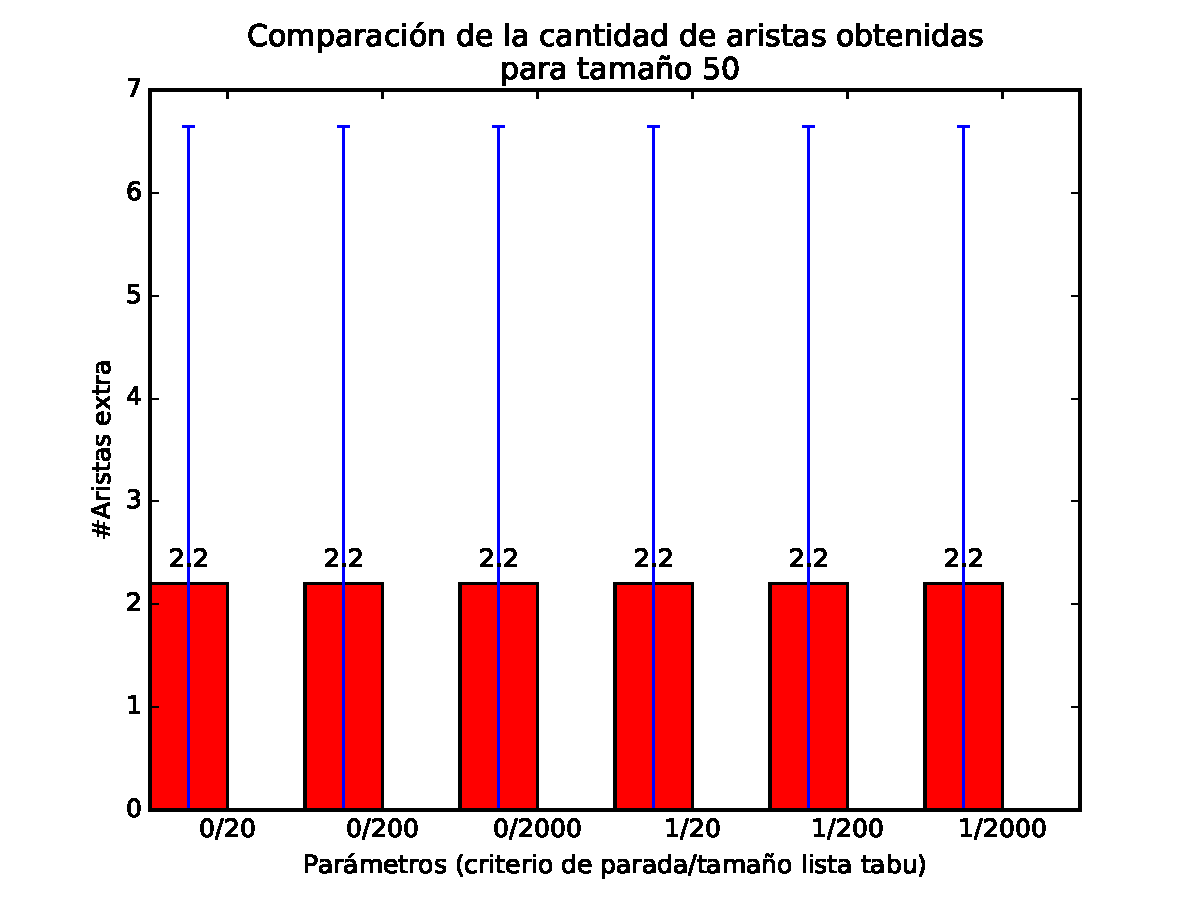
\includegraphics[width=1\textwidth]{graficos/problema_6/calidad0.pdf}
  \caption{\footnotesize{}}
  \label{fig:calidad5-1}
\end{minipage}%
\hspace{0.01\textwidth}
\begin{minipage}{0.49\textwidth}   
  \centering
    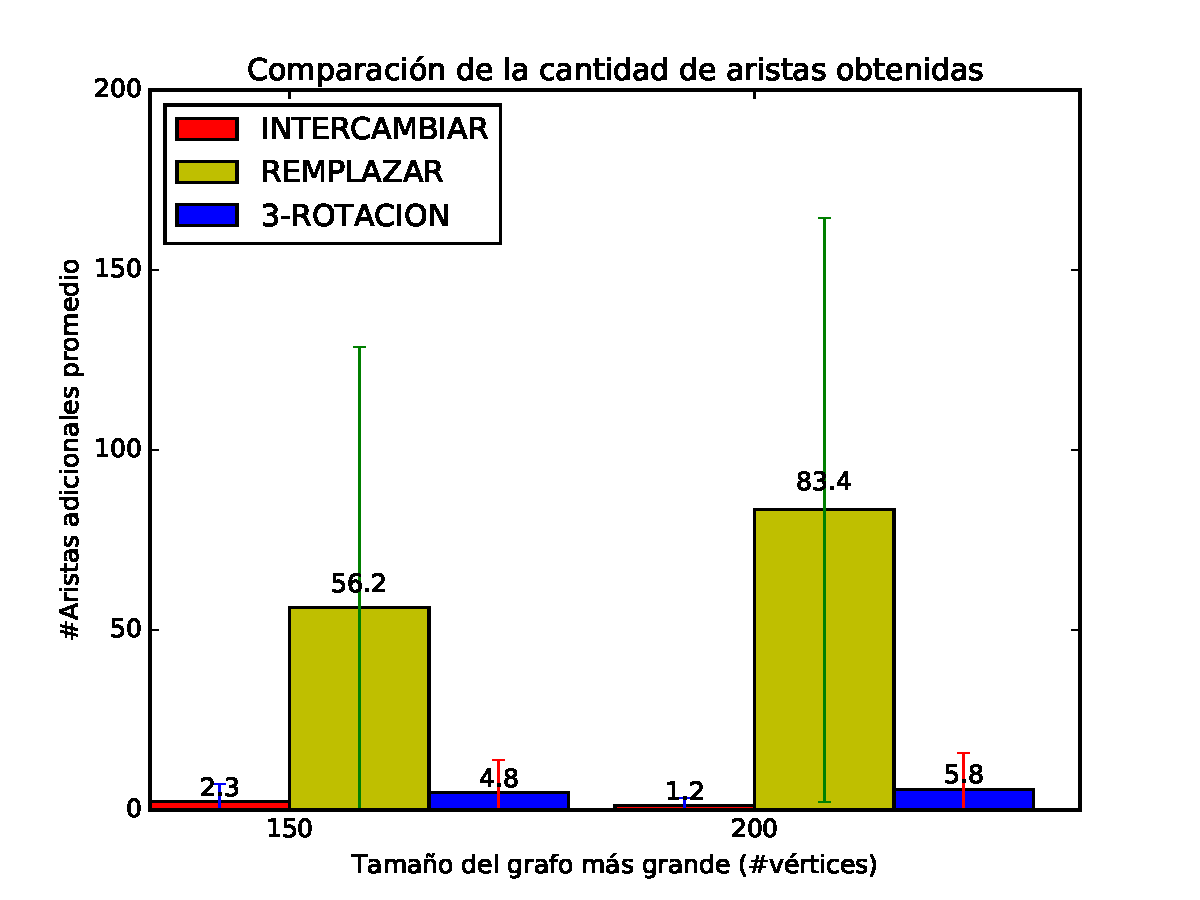
\includegraphics[width=1\textwidth]{graficos/problema_6/calidad2.pdf} 
  \caption{\footnotesize{}}
  \label{fig:calidad5-2}
\end{minipage}

\begin{minipage}{0.49\textwidth}
  \centering
    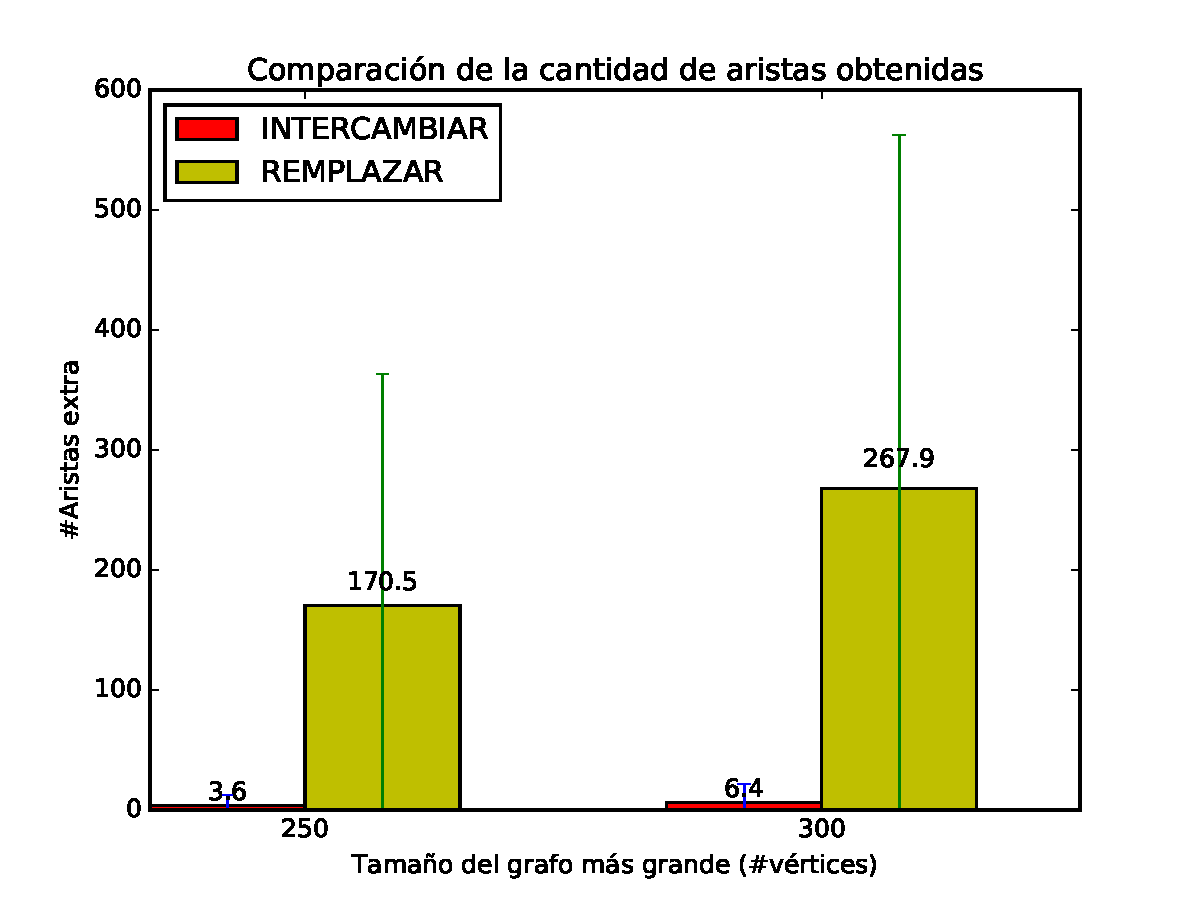
\includegraphics[width=1\textwidth]{graficos/problema_6/calidad4.pdf}
  \caption{\footnotesize{}}
  \label{fig:calidad5-3}
\end{minipage}%
\hspace{0.01\textwidth}
\begin{minipage}{0.49\textwidth}   
  \centering
    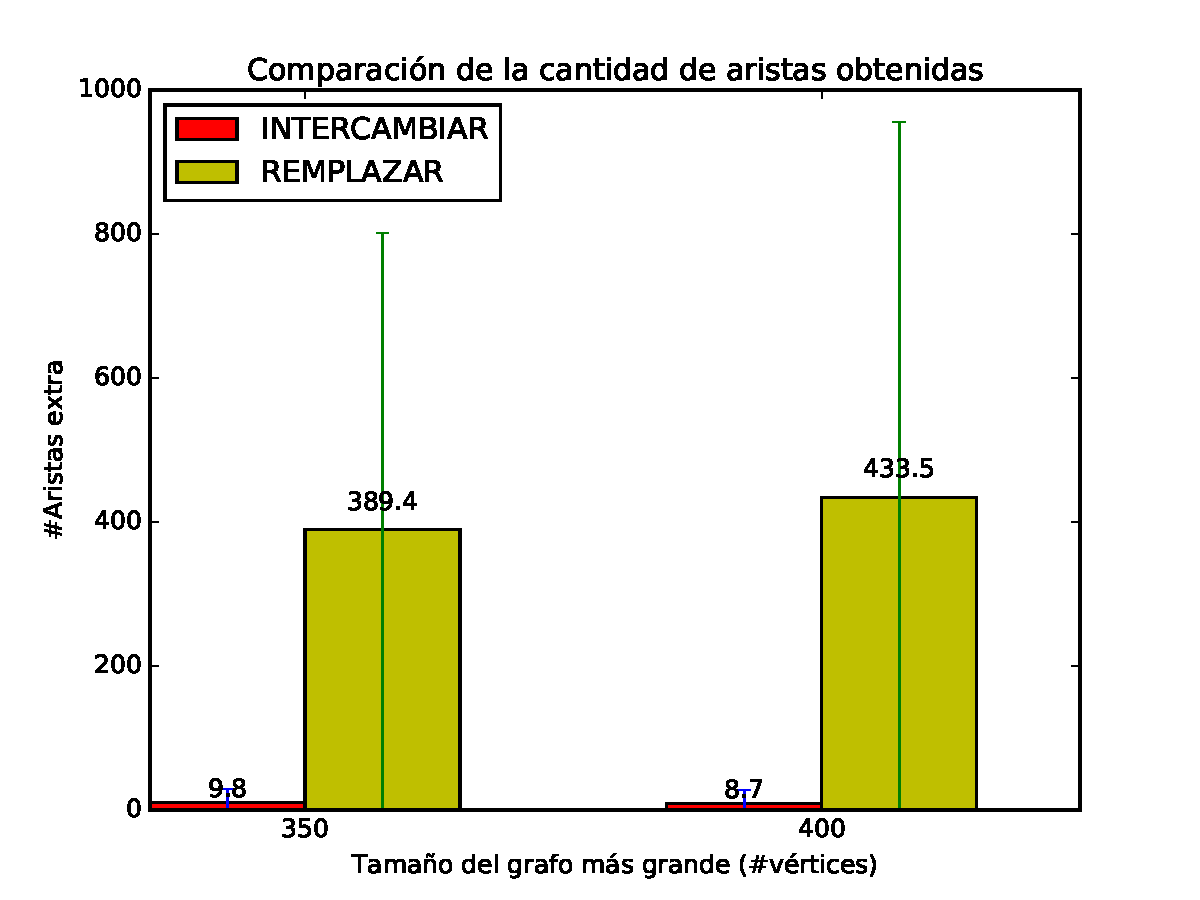
\includegraphics[width=1\textwidth]{graficos/problema_6/calidad6.pdf} 
  \caption{\footnotesize{}}
  \label{fig:calidad5-4}
\end{minipage}

\begin{minipage}{0.5\textwidth}   
  \centering
    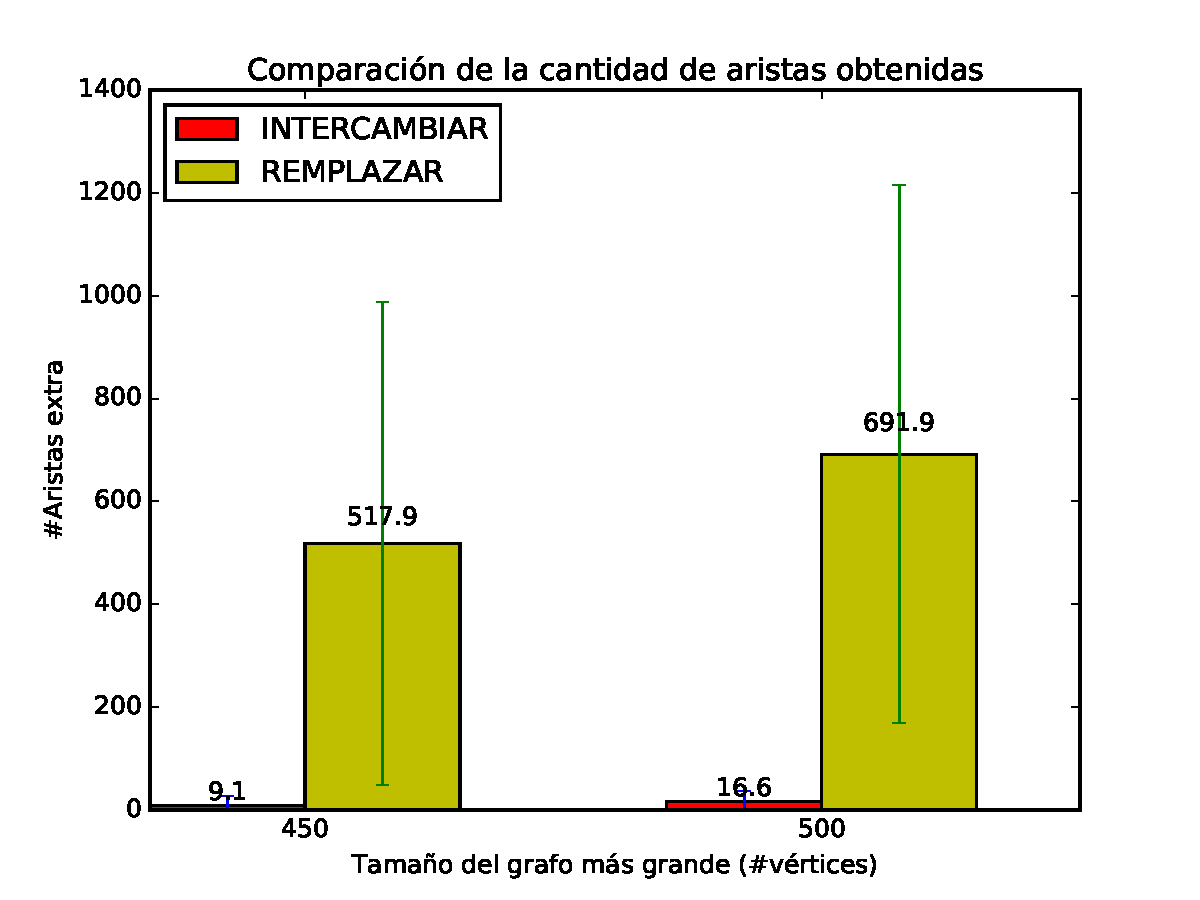
\includegraphics[width=1\textwidth]{graficos/problema_6/calidad8.pdf} 
  \caption{\footnotesize{}}
  \label{fig:calidad5-5}
\end{minipage}
\end{figure}


%%%%%Cociente%%%%%
\begin{figure}[H]
\centering
\begin{minipage}{0.49\textwidth}
  \centering
    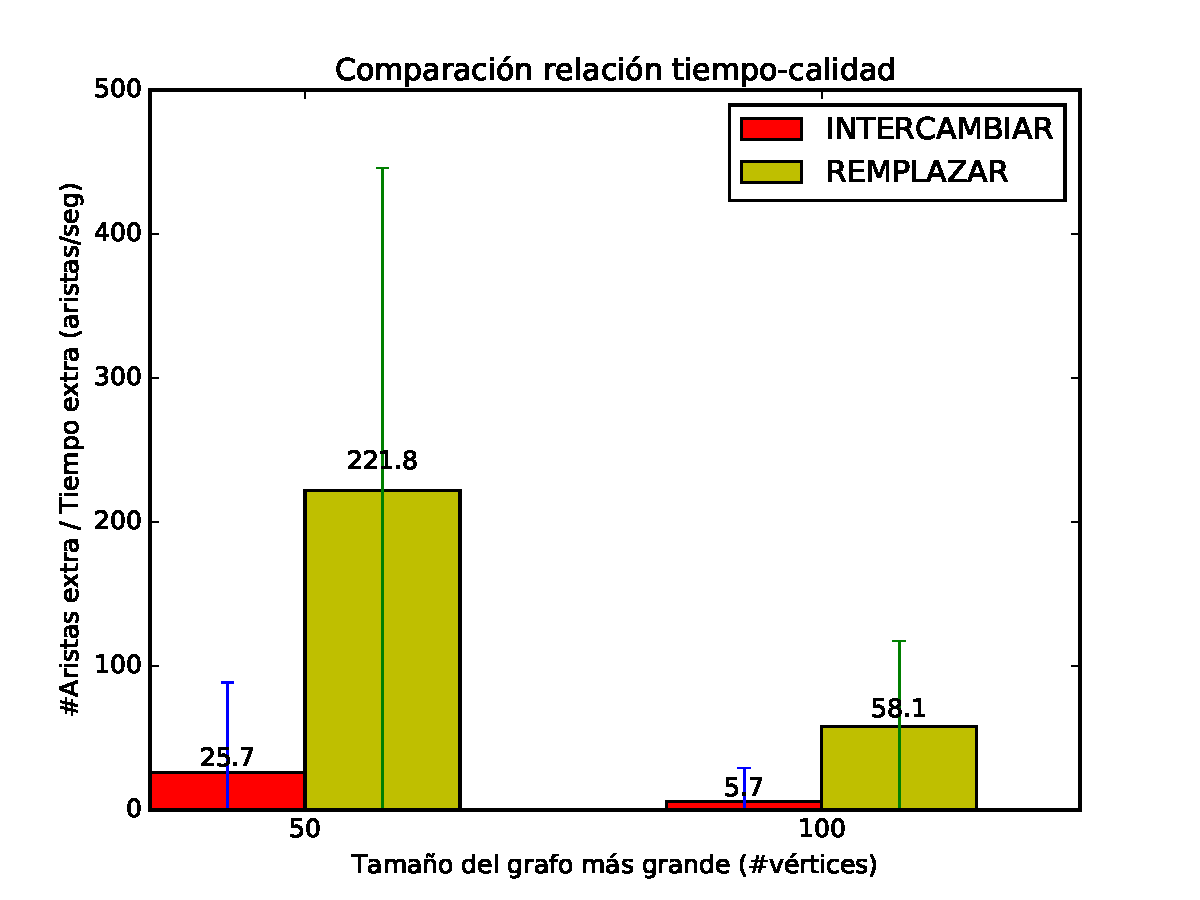
\includegraphics[width=1\textwidth]{graficos/problema_6/cociente0-0.pdf}
  \caption{\footnotesize{}}
  \label{fig:calidad5-1}
\end{minipage}%
\hspace{0.01\textwidth}
\begin{minipage}{0.49\textwidth}   
  \centering
    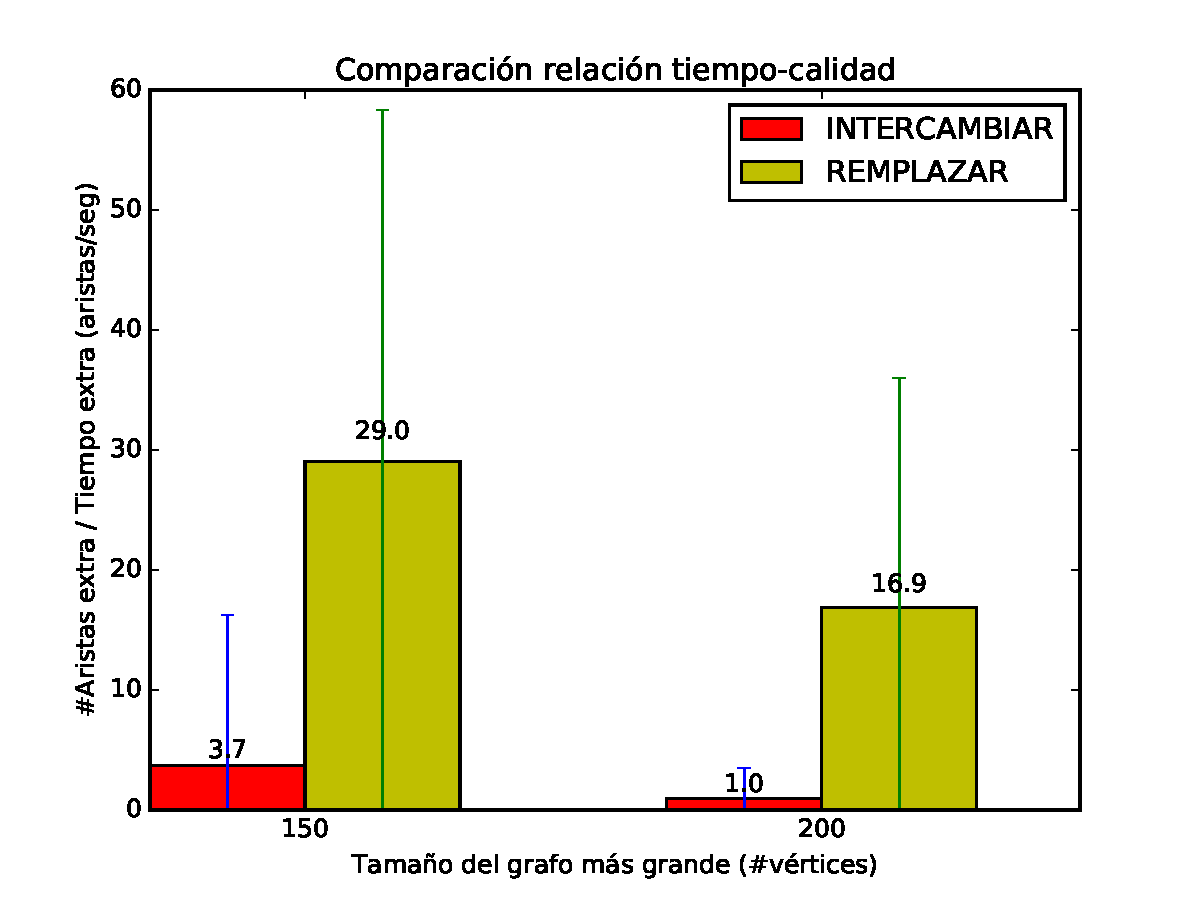
\includegraphics[width=1\textwidth]{graficos/problema_6/cociente0-2.pdf} 
  \caption{\footnotesize{}}
  \label{fig:calidad5-2}
\end{minipage}

\begin{minipage}{0.49\textwidth}
  \centering
    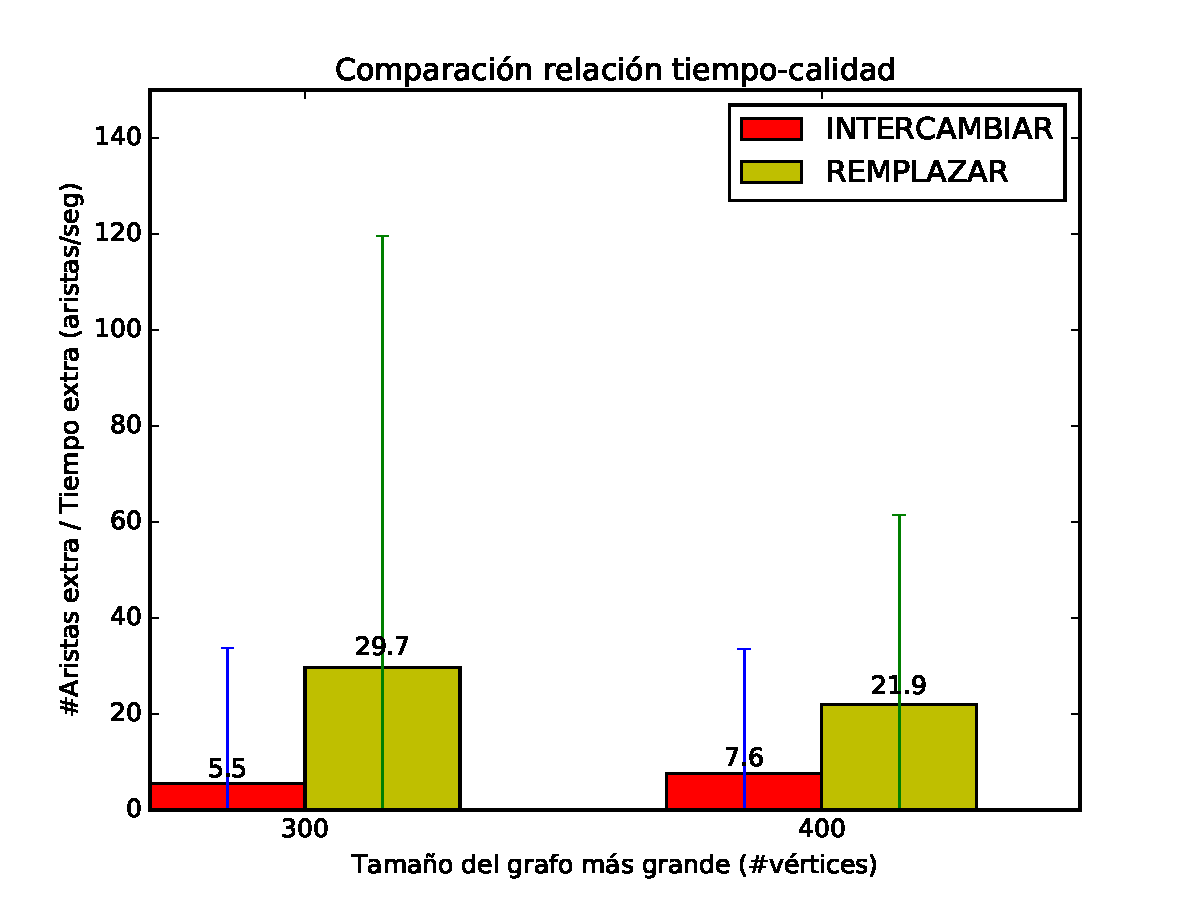
\includegraphics[width=1\textwidth]{graficos/problema_6/cociente0-4.pdf}
  \caption{\footnotesize{}}
  \label{fig:calidad5-3}
\end{minipage}%
\hspace{0.01\textwidth}
\begin{minipage}{0.49\textwidth}   
  \centering
    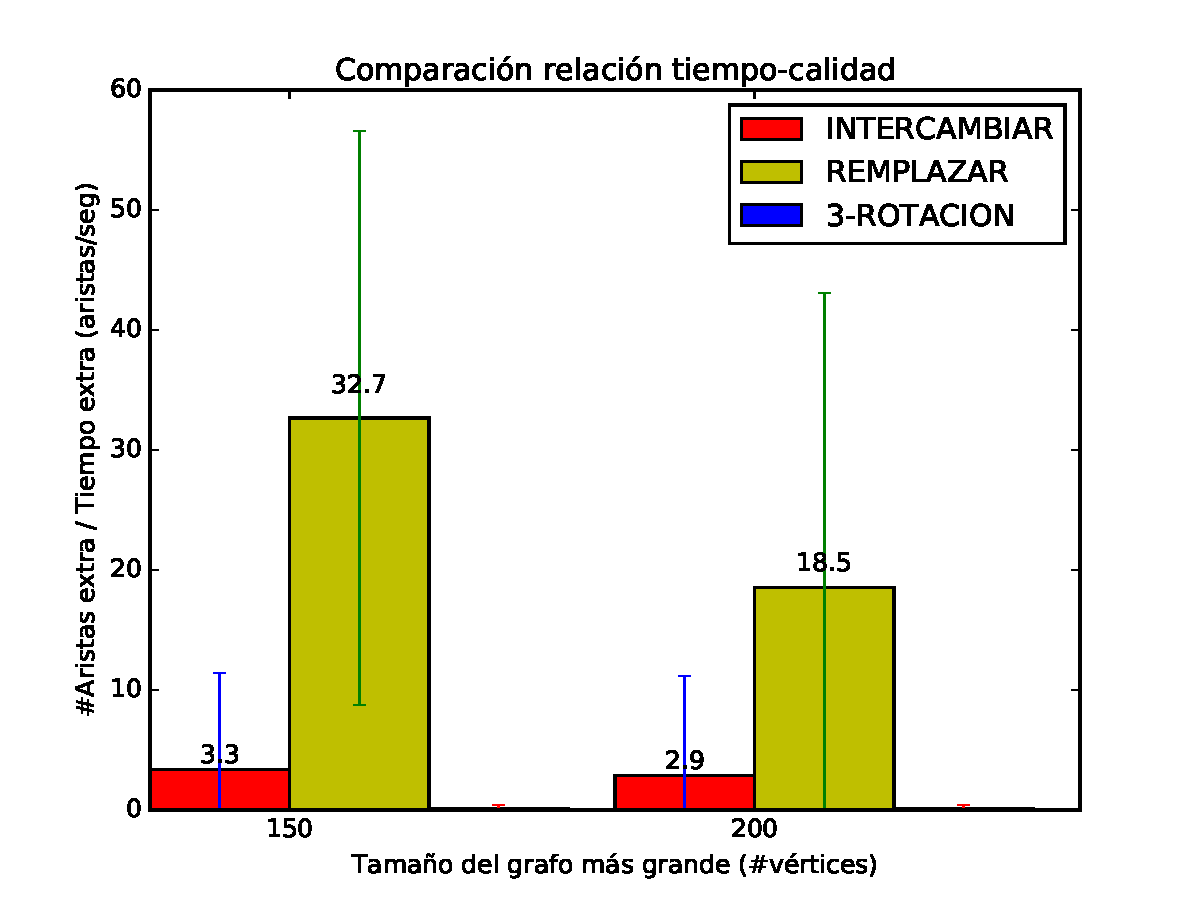
\includegraphics[width=1\textwidth]{graficos/problema_6/cociente1-2.pdf} 
  \caption{\footnotesize{}}
  \label{fig:calidad5-4}
\end{minipage}
\end{figure}


\begin{figure}[H]
  \centering
  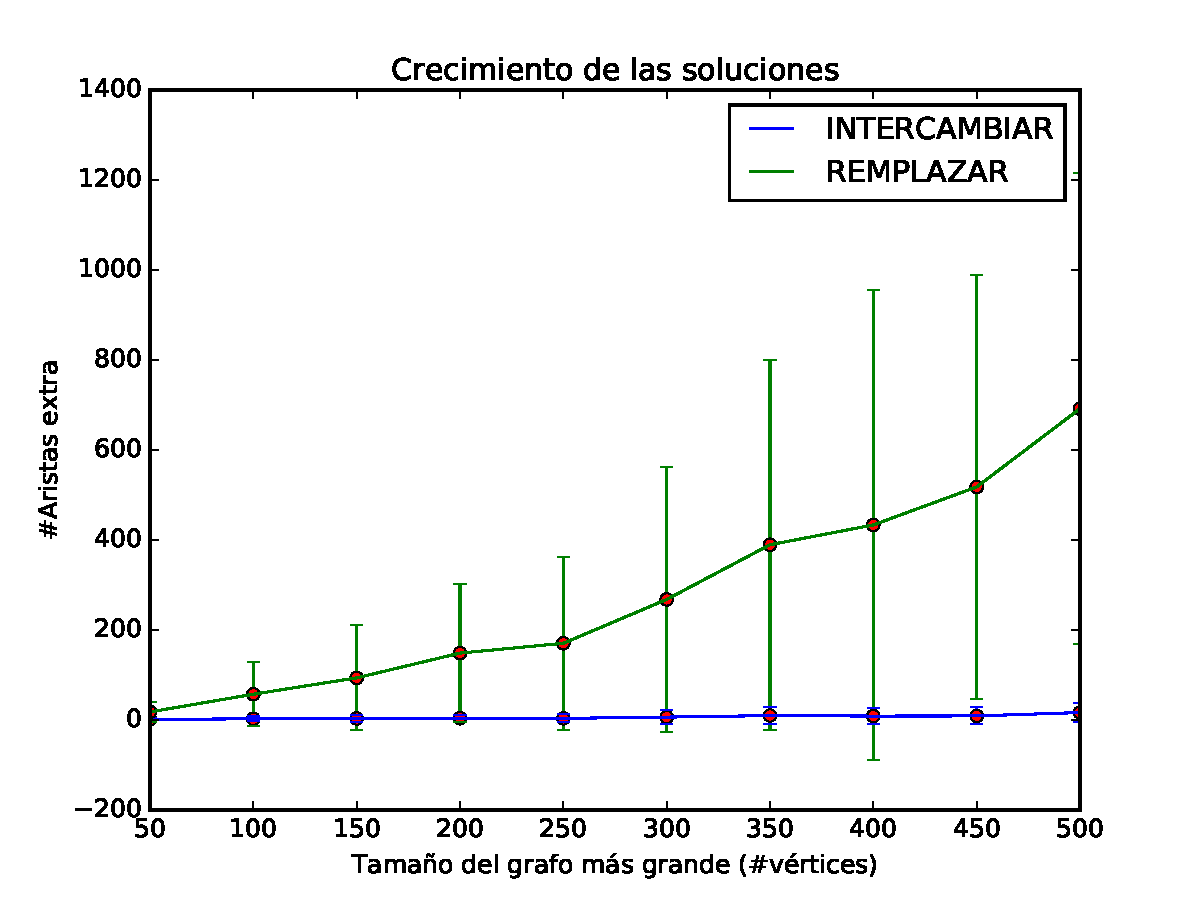
\includegraphics[width=1\textwidth]{graficos/problema_6/crecimiento.pdf} 
  \caption{\footnotesize{}}
  \label{fig:crecimiento}
\end{figure}